\section{Blender}
Blenderは, 3Dコンピュータグラフィックスやアニメーションを制作することができるオープンソースの3DCGソフトウェアである.
モデリング機能やテクスチャ機能など, 豊富な機能が備わっている.
また, Blender内に独立したPython環境が搭載されており, Python言語を使用して独自のスクリプトを作成することが可能となっている.
Blenderは商用のアニメーション映画にも利用されているほか, 建築の透視図やCADにも活用されている.

\vspace{5mm}
\begin{figure}[H]
     \centering
     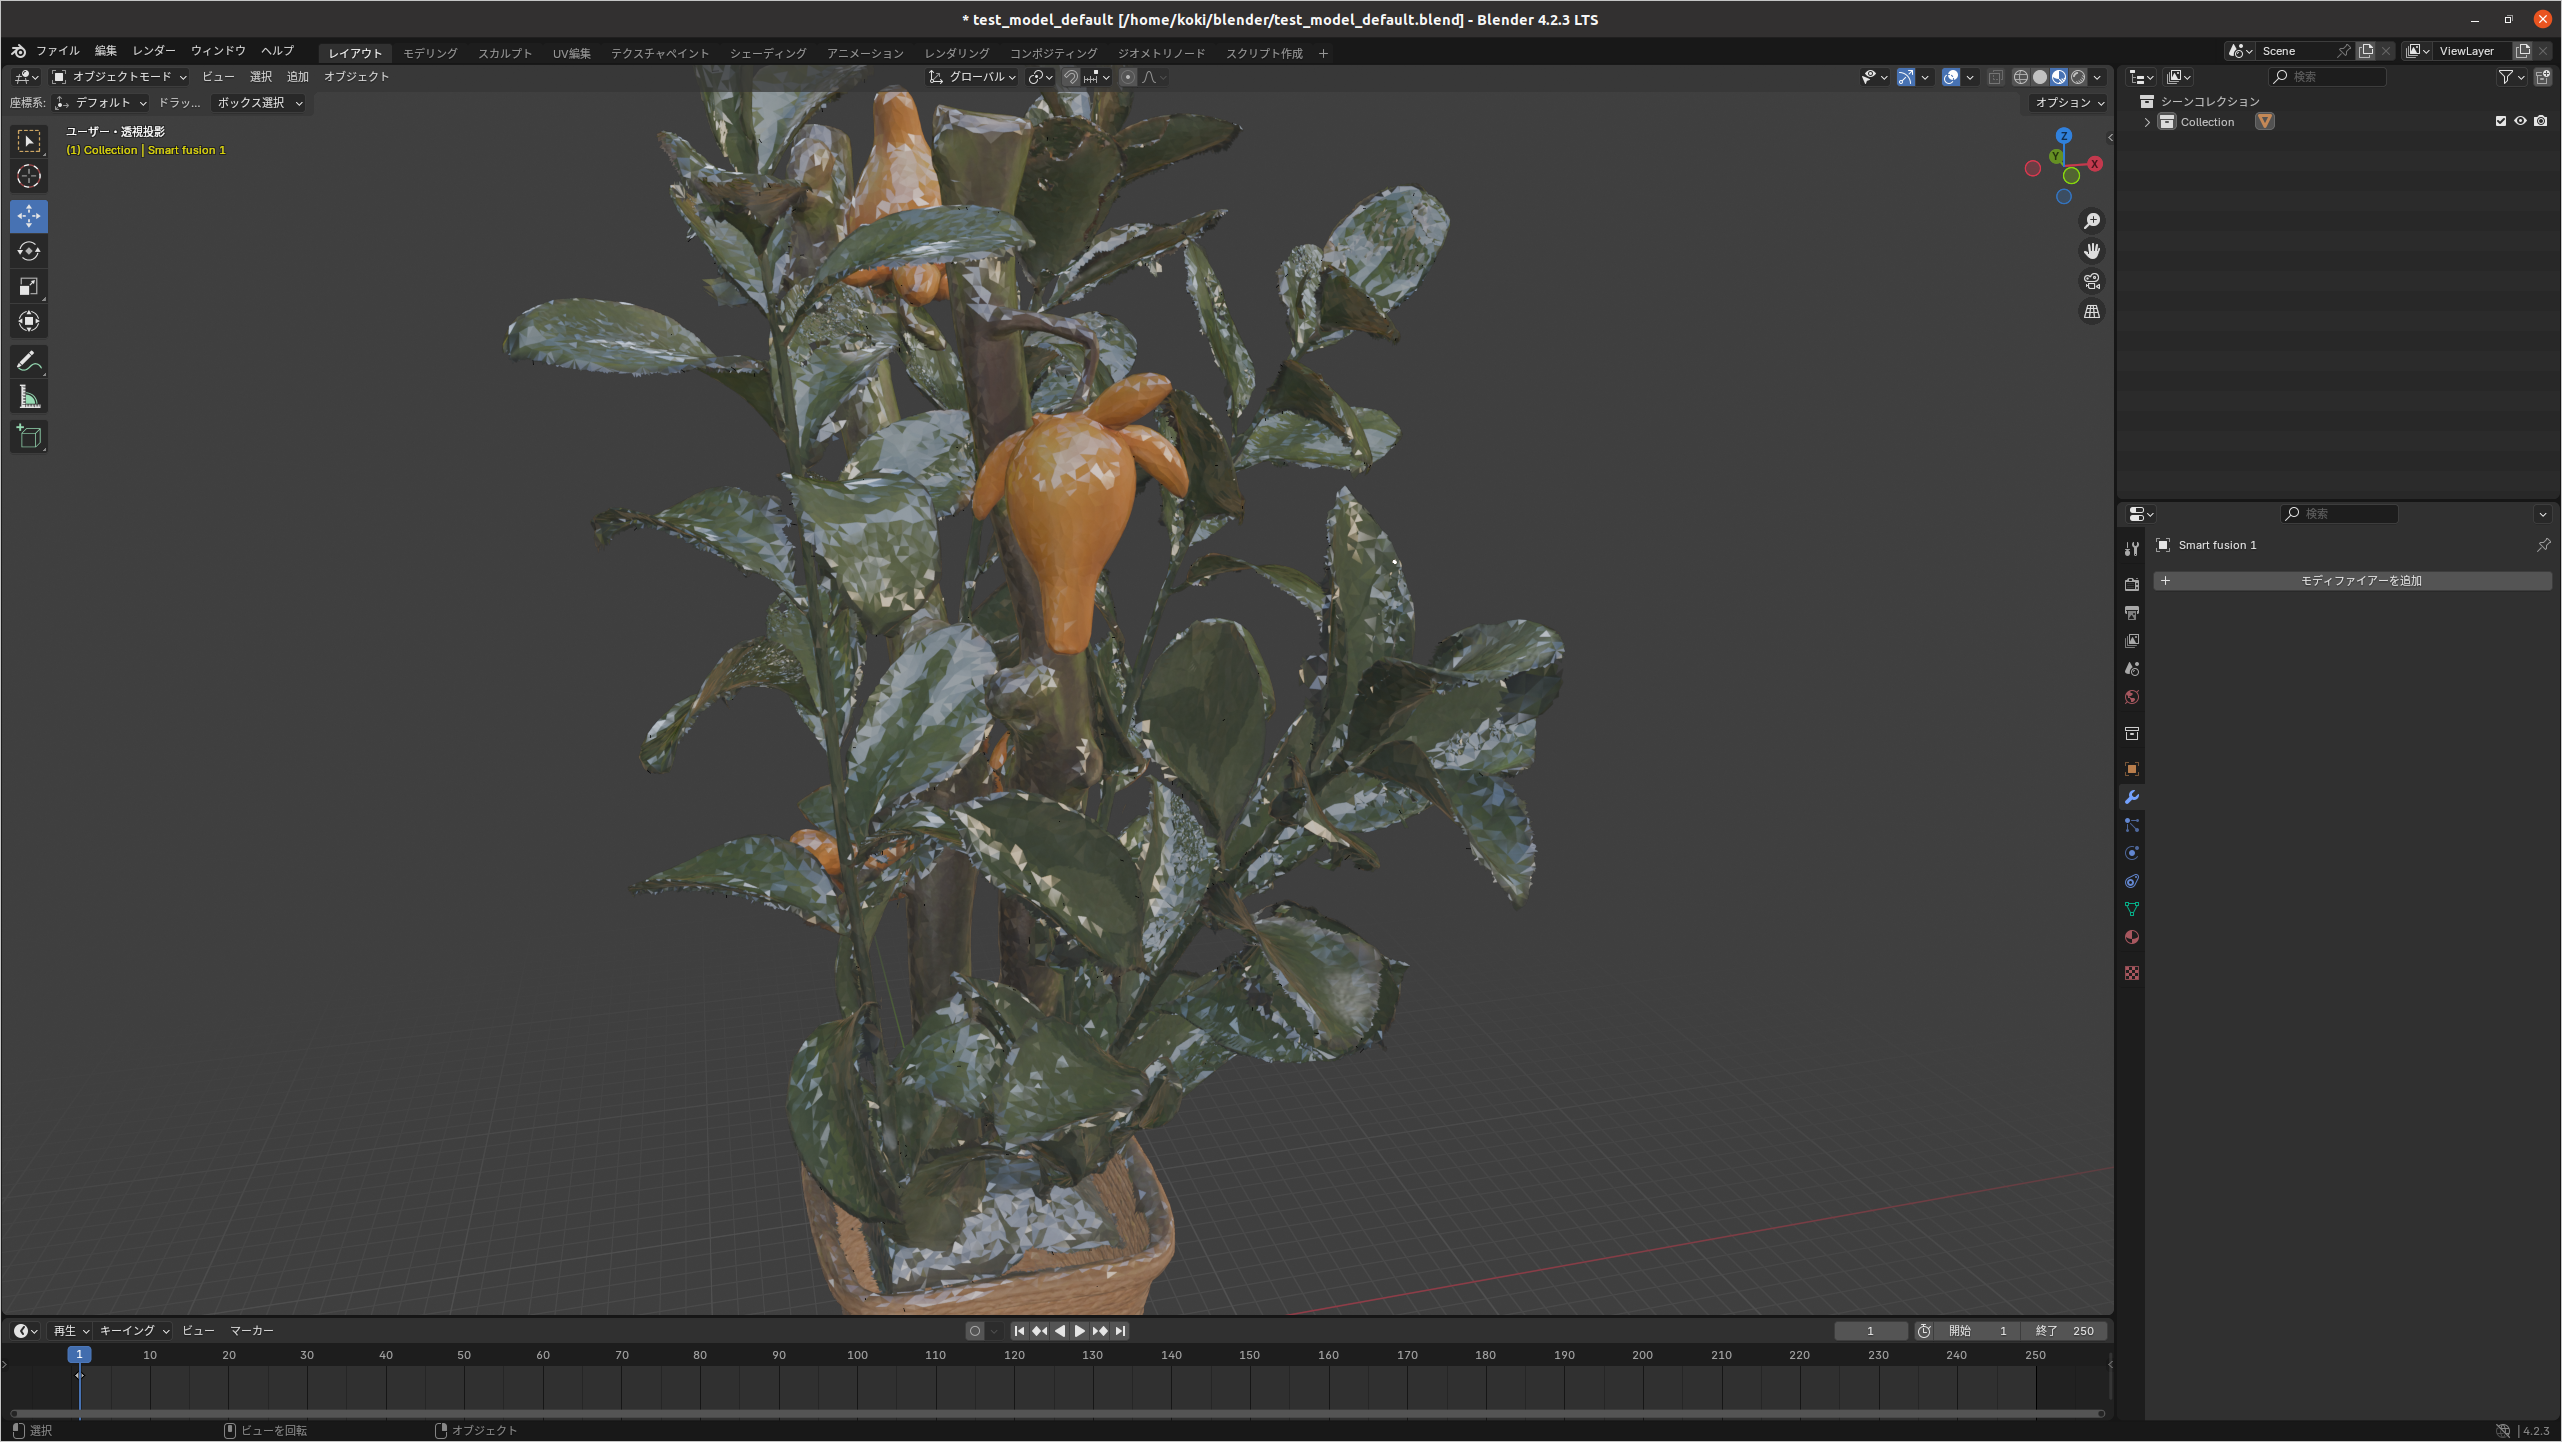
\includegraphics[width=110mm]{images/png/blenderex.png}
     \caption{Example Blender}
     \label{Fig:blenderex}
   \end{figure}